\documentclass[a4paper]{article}
\usepackage{cmap}
\usepackage[utf8]{inputenc}
\usepackage[T2A]{fontenc}
\usepackage[english,russian]{babel} 
\usepackage[left=15mm, top=15mm, right=15mm, bottom=42mm, nohead, nofoot]{geometry}
\usepackage{blindtext}  % рыба-текст
\usepackage{graphicx}  % изобржаения
\usepackage{float} % плавающие объекты
\usepackage{wrapfig}  % изобржаения
\usepackage{tikz} % графика
\usepackage{mdframed} % рамки
\usepackage{xcolor} % определение цветов
\usepackage{nicefrac} % красивые дроби
\usepackage{cancel} % сокращение
\usepackage{amsmath,amsfonts,amssymb} % математический пакет
\usepackage{hyperref}  % гиперссылки
\usepackage{fancybox,fancyhdr} % хедер и футер
\usepackage{listings} % код
\pagestyle{fancy}
\fancyhf{}
\fancyhead[L]{Домашнее задание №1}
\fancyhead[R]{Теория вероятностей}
\fancyfoot[C]{\thepage}
\headsep=8mm
\footskip=20mm

\definecolor{urlcolor}{HTML}{3454D1}
\definecolor{linkcolor}{HTML}{3454D1}
\hypersetup{pdfstartview=FitH, linkcolor=linkcolor, urlcolor=urlcolor, colorlinks=true}
\definecolor{strings}{rgb}{0,0.6,0}
\definecolor{comments}{rgb}{0,0.3,0}
\definecolor{numbers}{rgb}{0.5,0.5,0.5}
\definecolor{keywords}{rgb}{0.09,0.61,0.95}
\definecolor{background}{rgb}{0.97,0.97,0.97}
\lstdefinestyle{codestyle}{
    backgroundcolor=\color{background},
    commentstyle=\color{comments},
    keywordstyle=\color{keywords},
    stringstyle=\color{strings},
    numberstyle=\tiny\color{numbers},
    basicstyle=\ttfamily\footnotesize,
    breakatwhitespace=false,
    breaklines=true,
    captionpos=b,
    inputencoding=utf8,
    keepspaces=true,
    numbers=left,
    numbersep=5pt,
    showspaces=false,
    showstringspaces=false,
    showtabs=false,
    tabsize=2,
    extendedchars=true,
    literate=
    {а}{{\cyra}}1
    {б}{{\cyrb}}1
    {в}{{\cyrv}}1
    {г}{{\cyrg}}1
    {д}{{\cyrd}}1
    {е}{{\cyre}}1
    {ж}{{\cyrzh}}1
    {з}{{\cyrz}}1
    {и}{{\cyri}}1
    {й}{{\cyrishrt}}1
    {к}{{\cyrk}}1
    {л}{{\cyrl}}1
    {м}{{\cyrm}}1
    {н}{{\cyrn}}1
    {о}{{\cyro}}1
    {п}{{\cyrp}}1
    {р}{{\cyrr}}1
    {с}{{\cyrs}}1
    {т}{{\cyrt}}1
    {у}{{\cyru}}1
    {ф}{{\cyrf}}1
    {х}{{\cyrh}}1
    {ц}{{\cyrc}}1
    {ч}{{\cyrch}}1
    {ш}{{\cyrsh}}1
    {щ}{{\cyrshch}}1
    {ъ}{{\cyrhrdsn}}1
    {ы}{{\cyrery}}1
    {ь}{{\cyrsftsn}}1
    {э}{{\cyrerev}}1
    {ю}{{\cyryu}}1
    {я}{{\cyrya}}1
    {А}{{\CYRA}}1
    {Б}{{\CYRB}}1
    {В}{{\CYRV}}1
    {Г}{{\CYRG}}1
    {Д}{{\CYR96}}1
    {Е}{{\CYRE}}1
    {Ж}{{\CYRZH}}1
    {З}{{\CYRZ}}1
    {И}{{\CYRI}}1
    {Й}{{\CYRISHRT}}1
    {К}{{\CYRK}}1
    {Л}{{\CYRL}}1
    {М}{{\CYRM}}1
    {Н}{{\CYRN}}1
    {О}{{\CYRO}}1
    {П}{{\CYRP}}1
    {Р}{{\CYRR}}1
    {С}{{\CYRS}}1
    {Т}{{\CYRT}}1
    {У}{{\CYRU}}1
    {Ф}{{\CYRF}}1
    {Х}{{\CYRH}}1
    {Ц}{{\CYRC}}1
    {Ч}{{\CYRCH}}1
    {Ш}{{\CYRSH}}1
    {Щ}{{\CYRSHCH}}1
    {Ъ}{{\CYRHRDSN}}1
    {Ы}{{\CYRERY}}1
    {Ь}{{\CYRSFTSN}}1
    {Э}{{\CYREREV}}1
    {Ю}{{\CYRYU}}1
    {Я}{{\CYRYA}}1
}

\lstset{style=codestyle}

\addto\captionsrussian{
  \renewcommand{\contentsname}
    {\centering Содержание}
}
\newcommand{\addsection}[1]{
    \phantomsection
    \addcontentsline{toc}{section}{#1}
    \section*{\centering #1}
}
\newcommand{\addsubsection}[1]{
    \phantomsection
    \addcontentsline{toc}{subsection}{#1}
    \subsection*{\centering #1}
}
\newcommand{\addsubsubsection}[1]{
    \phantomsection
    \addcontentsline{toc}{subsubsection}{#1}
    \subsubsection*{\centering #1}
}

\newmdenv[
  leftmargin = 0.5em,
  skipabove = 0.5em,
  skipbelow = 0.5em,
  linewidth = 1pt,
  rightline = false,
  topline = false,
  bottomline = false
]{quotebox}

\newlength{\tempheight}
\newcommand{\Let}{
\mathbin{\text{\settoheight{\tempheight}{\mathstrut}\raisebox{0.4\pgflinewidth}{
\tikz[baseline=0.5ex,line cap=round,line join=round] \draw (0,0) --++ (0.3em,0) --++ (0,2.3ex) --++ (-0.3em,0);
}}}}
\newcommand*\squared[1]{\tikz[baseline=(char.base)]{
            \node[shape=rectangle,draw,inner sep=4pt] (char) {#1};}}
\newcommand*\msquared[1]{\tikz[baseline=(char.base)]{
            \node[shape=rectangle,draw,inner sep=4pt] (char) {$\displaystyle #1$};}}
\newcommand{\at}{\biggr\rvert}
\newcommand{\shiftright}[3]{\makebox[#2][r]{\makebox[#1][l]{#3}}}
\newcommand{\e}{\;\text{e}}
\let\oldint\int
\def\int{\oldint\limits}
\DeclareRobustCommand{\divby}{%
  \mathrel{\vbox{\baselineskip.65ex\lineskiplimit0pt\hbox{.}\hbox{.}\hbox{.}}}%
}

\newcommand\NB{\textbf{N\kern-0.32em\textcolor{red}{B}}}

\begin{document}
\begin{titlepage}
    \begin{center}
        Федеральное государственное автономное образовательное \\ учреждение высшего образования \\[6pt]
        САНКТ-ПЕТЕРБУРГСКИЙ НАЦИОНАЛЬНЫЙ \\ ИССЛЕДОВАТЕЛЬСКИЙ УНИВЕРСИТЕТ ИТМО \\[16pt]
        Факультет систем управления и робототехники \\[26em]
        \Large{\textbf{Домашнее задание №1}} \\
        \Large{\textbf{по теории вероятностей}}
    \end{center}\,\\[9em]
    \begin{flushright}
        Студент: Овчинников П.А.\\
        ИСУ: 368606 (вариант №3)\\
        Поток: ТеорВер 1.2 \\[0.5em]
        Преподаватели: Шиманская Г.С.\\
        Ватутин А.Д.
    \end{flushright}\,\\[6em]
    \begin{center}
        {\small Санкт-Петербург \\ 2024}
    \end{center}
\end{titlepage}
\setcounter{page}{2}
\noindent Имеется 8 баллов за работу на занятиях, следовательно могу сделать всего лишь 3 задания в домашней работе, чтобы получить максимальные 20 баллов за первый раздел дисциплины.
% MARK: Задание №1
\addsection{Задание №1}
Рассмотрим каждое из событий по отдельности под призмой теоремы о вписанном угле:
\begin{enumerate}
    \item $\angle ABC$ острый --- на величину угла влияют точки $A$ и $C$,смещение точки $B$ не изменяет его величину по теореме о вписанном угле.
    \item $\angle ACB$ острый --- на величину угла влияют точки $A$ и $B$, смещение точки $C$ не изменяет его величину по теореме о вписанном угле.
\end{enumerate}
Если бы точки $B$ и $C$ были зафиксированы и произвольным было бы только положение $A$, то тогда можно было бы говорить о зависимости событий, но в нашем случае \underline{события независимы}, т.к. кроме $A$ в этих двух углах их величины задают другие две точки, которые выбираются произвольно и независимо.\\[1em]
Теперь воспользуемся теоремой Фалеса, которая сообщает нам, что угол, опирающий на диаметр окружности, всегда прямой. Рассмотрим $\vartriangle ABC$ (рис. 1):
\begin{figure}[H]
    \begin{minipage}{0.44\textwidth}
        \centering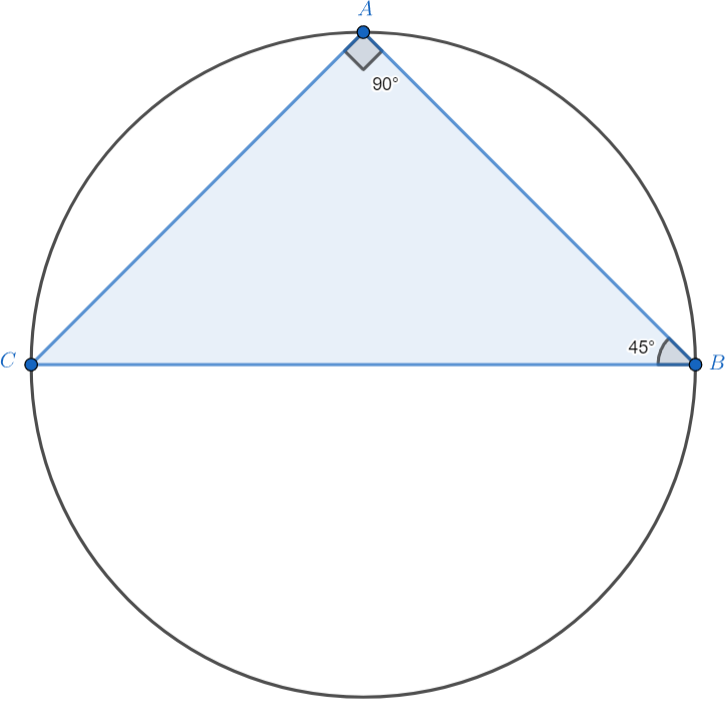
\includegraphics[width=\textwidth]{start.png}
        \caption{Начальное состояние $\vartriangle ABC$}
    \end{minipage}\hfill
    \begin{minipage}{0.44\textwidth}
        \centering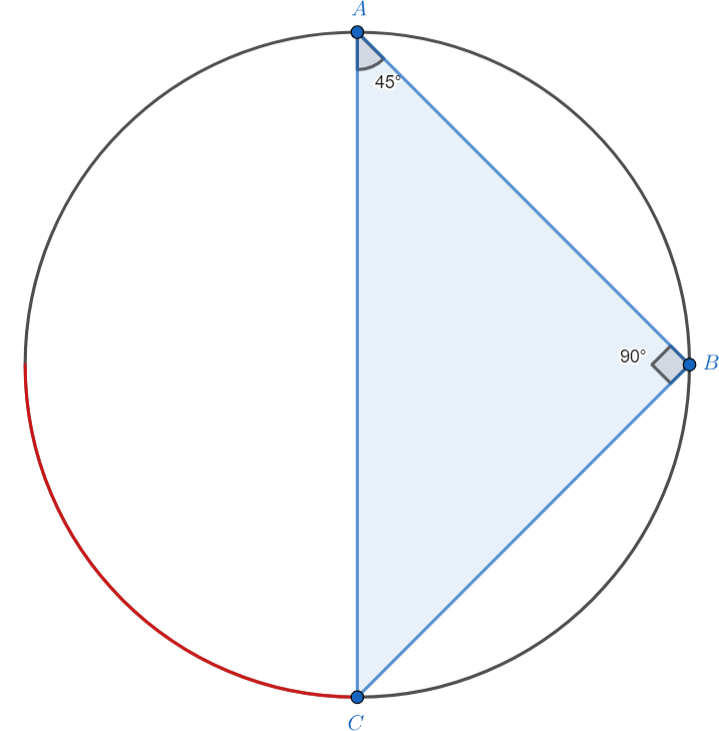
\includegraphics[width=\textwidth]{finish.png}
        \caption{Конечное состояние $\vartriangle ABC$}
    \end{minipage}
\end{figure}
\noindent Отметим $\angle A$ и $\angle B$, чтобы видеть, как они изменяются, и будем двигать точку $C$ против часовой стрелки до тех пор, пока отрезок $AC$ не станет параллельным вертикальной оси. Во время этого движения заметим, что:
\begin{itemize}
    \item $\angle C$ остаётся неизменным по теореме о вписанном угле, т.к. опирается на одну и ту же прямую,
    \item $\angle A$ будет уменьшаться от $90^\circ$ до $45^\circ$,
    \item $\angle B$ будет, наоборот, увеличиваться от $45^\circ$ до $90^\circ$.
\end{itemize}
Во время всего этого движения треугольник будет остроугольным, т.к. все углы будут острые (не учитывая крайние состояния, когда треугольник опирается на диаметр и $\angle A = 90^\circ$ или $\angle B = 90^\circ$). Когда точка $C$ закончит движение, мы вновь получим прямоугольный треугольник теперь уже с прямым $\angle B$. При дальнейшем движении точки $C$ мы получим тупоугольный треугольник с $\angle$.На рис. 2 выделена дуга, по которой двигалась точка $C$ --- она составляет \msquared{\nicefrac{1}{4}} от общей длины окружности. Это и есть ответ.\\[1em]
Возвращаясь к теореме о вписанно угле и рассматривая начальное состояние, мы также можем двигать точку $A$ от точки $C$ до точки $B$ и получим дугу, равную половине окружности --- на всей этой дуге треугольник будет прямоугольный и $\angle A$ будет равне $90^\circ$. Получаем ответ на вторую часть задания --- \msquared{\nicefrac{1}{2}}.

% MARK: Задание №3
\addsection{Задание №3}
Вспомним формулу условной вероятности: $P(X|Y) = \frac{P(X\cdot Y)}{P(X)}$. Согласно этой формуле раскроем выражение из условия задания:
$$P(A|B) + P(A|\bar{B}) = \frac{P(A\cdot B)}{P(B)} + \frac{P(A\cdot \bar{B})}{P(\bar{B})}$$
Предположим, что события независимые. В таком случае, как мы знаем, для двух независмых событий верно равенство $P(X\cdot Y) = P(X)\cdot P(Y)$. Согласно этой формуле получаем:
$$\frac{P(A\cdot B)}{P(B)} + \frac{P(A\cdot \bar{B})}{P(\bar{B})} = \frac{P(A)\cdot \cancel{P(B)}}{\cancel{P(B)}} + \frac{P(A)\cdot \cancel{P(\bar{B})}}{\cancel{P(\bar{B})}} = P(A) + P(A) = P(A)$$
$P(A) = P(A|B) + P(A|\bar{B}) = P(A) \Rightarrow$ наше предположение верно, и \underline{события действительно независимые}.

% MARK: Задание №5
\addsection{Задание №5}
Пусть имеются три события:
\begin{itemize}
    \item $S_1$ --- первым произвёл выстрел первый стрелок
    \item $S_2$ --- первым произвёл выстрел второй стрелок
    \item $A$ --- при пятом выстреле произошло попадание в мишень
\end{itemize}
Вероятность, которую мы ищем --- $P(S_1|A)$. Раскроем её по формуле Байеса: $P(S_1|A) = \frac{P(S_1)P(A|S_1)}{P(A)}$. Необходимо найти каждое неизвестное в формуле.\\[1em]
Начнём с того, что вероятность первых двух событий равна, то есть $P(S_1) = P(S_2) = 0.5$, потому как доподлинно неизвестно, кто начал первым и в равной степени это мог быть как первый стрелок, так и второй.\\[0.5em]
Теперь найдём вероятность события $A$ при условии возникновения событий $S_1$ или $S_2$:
$$P(A|S_1) = (1 - 0.4)\cdot(1 - 0.5)\cdot(1-0.45)\cdot(1-0.55)\cdot0.5 = 0.6\cdot0.5\cdot0.55\cdot0.45\cdot0.5 = \frac{297}{8000}$$
$$P(A|S_2) = (1 - 0.5)\cdot(1-0.4)\cdot(1-0.55)\cdot(1-0.45)\cdot0.6 = 0.5\cdot0.6\cdot0.45\cdot0.55\cdot0.6 = \frac{891}{20000}$$
И воспользуемся формулой полной вероятности, чтобы найти $P(A)$:
$$P(A) = P(S_1)P(A|S_1) + P(S_2)P(A|S_2) = \frac{1}{2}\cdot\frac{297}{8000} + \frac{1}{2}\cdot\frac{891}{20000} = \frac{1}{2}\left( \frac{297}{8000} + \frac{891}{20000} \right) = \frac{1}{2}\cdot\frac{3267}{40000} = \frac{3267}{80000}$$
Все слагаемые для нахождения искомой вероятности имеются, найдём же её:
$$P(S_1|A) = \frac{P(S_1)P(A|S_1)}{P(A)} = \frac{\frac{1}{2}\cdot\frac{297}{8000}}{\frac{3267}{80000}} = \frac{\cancelto{5}{80000}\;\cdot297}{\cancel{16000}\cdot3267} = \frac{1485}{3267} \approx \msquared{0.(45)}$$

\end{document}